\section{Experimental Evaluation}
\label{sec:eval}
The evaluation examines configured protocol and node access, entry-specific
records, approval-context checks, and control requests and observations during
optimization. Protocol connectivity and
four optimization missions were recorded on September 28, 2026. The missions
cover injection molding, biaxially oriented polyethylene terephthalate
(BOPET) film production, continuous annealing, and anaerobic/anoxic/oxic
wastewater treatment. A separate later onboarding replay and mock-state
approval test and two entry-path checks examine separate integration mechanisms;
they are not additional trials of the four missions. Table~\ref{tab:missions}
summarizes the process values, and Fig.~\ref{fig:missions} shows the recorded
intermediate observations.

\subsection{Test Design and Interpretation}
\label{sec:eval-protocol}
The missions ran against locally configured process simulators, using a
deterministic scenario-specific control routine and a fixed random seed.
The routines inspected process values and requested bounded control changes.
The available benchmark source records an automatic keep judgment after a
write returned, before the subsequent process observation; its BOPET routine
judges after observing the response. The full executed runtime snapshot was
not retained. Annealing and wastewater logs also contain subsequent explicit
reversion decisions. These judgments are software events, not evidence of
human pre-approval.
The records use the direct-node operation interface; they do not exercise all
task-entry routes or use a language model to select setpoints. Protocol drivers
communicated with simulator endpoints rather than physical equipment.
These archived missions illustrate their recorded operation--observation
sequence; they do not verify every feature of the architecture described in
Sections~\ref{sec:design} and~\ref{sec:modules}.

Each scenario contributes one trajectory. Its initial observation is the
within-trajectory reference, not an independent control group. A requested
setpoint is an action, whereas a subsequent process value is an observation;
the former should not be read as a device readback. The primary outcome is
whether the reported final value lies inside the scenario's stated target
band. Intermediate observations provide context for the sequence, but are
not independent repetitions, and the event positions in the figure indicate
order rather than elapsed time.

\subsection{Protocol and Node Integration}
The September protocol test configured local simulator endpoints using Modbus
TCP, Modbus RTU, OPC UA, MQTT, and HTTP. Its contemporaneous report records a
successful connectivity check for each protocol. In a Modbus TCP closed-loop
check, seven samples were collected and a 182\,$^{\circ}$C setpoint was
requested; the simulated process reached within 3\,$^{\circ}$C of that value
after 24\,s. In a separate fault case, a 185\,$^{\circ}$C write was read back
while the process value remained frozen at 150\,$^{\circ}$C; monitoring raised
an alarm within 2\,s. The reported link-fault exercise detected loss of
connection and recovered after the simulator restarted. These observations
distinguish protocol access and setpoint readback from the later process
response. They are from the contemporaneous summary, not a retained complete
per-sample protocol trace, and do not establish physical-device behavior.

The BOPET mission used a configured simulated line with nine devices and 49
signals: 30 writable setpoints and 19 measurements. Its four write requests
addressed three control nodes. A separate onboarding replay on October 26
instantiated one simulated Modbus TCP device with four write nodes and seven
acquisition nodes, together with scalar, vector, table, and image forms from a
manufacturing execution system (MES) simulator. The verifier found samples
for all seven acquisition nodes, rejected all four out-of-range writes, and
confirmed four legal writes by readback; its 23 checks passed. A test-only
automatic approval allowed a line-speed change from 37 to 39\,m/min, confirmed
by the simulator. This single replay demonstrates the configured integration
instance, not arbitrary protocol coverage or repeatability. Its source build
was not completely pinned, and the MES image used a local storage fallback.

\subsection{Task and Direct-Operation Entries}
Two separate simulator checks on October 25 exercised a fixed-call registered
task and a direct REST operation in each of two scenes. Each issued a recipe
trial with synthetic approval and returned a readback-verified receipt and a
run-tagged sample. The task route also retained a task--approval--receipt--sample
link, although task completion was not asserted; the direct route created no
task. Both used the same requested settings, but separate environments. After
20\,s, the task and direct samples were both 46.37\,$\mu$m for film thickness
and 674.80 and 675.20\,$^{\circ}$C, respectively, for annealing temperature;
all were below their respective 48--52\,$\mu$m and 700--760\,$^{\circ}$C
target bands. Each sample was an explicit driver probe stored using a local
database fallback with online DAQ collection disabled. These are single probes,
not response trajectories, online-pipeline validation, or evidence of
attainment. The runs show the records
available through each tested entry; they do not establish equivalent
behavior or directly trace both calls to the same handler. They are separate
from the September optimization missions.

\subsection{Approval Context and Dispatch}
An independent component test exercised human-in-the-loop (HITL) approval
using simulated decisions and a mock driver. A proposal binds the line,
product, recipe, and active run to the approval context; after approval the
handler compares that context with the current one before dispatch. The test
changed each of the four fields for recipe application, trial, and rollback:
all injected stale contexts were refused before mock writes. A further injected
change between authorization revalidation and the final check was also
refused. An unchanged approved context produced the expected mock writes,
whereas a rejected proposal produced none.

To examine the contribution of the context comparison, a test-only ablation
removed that comparison while retaining the other checks. Six product or run
changes then reached the mock driver and each produced two writes and an
execution record. The remaining six line or recipe changes were still blocked
by other checks. Thus the comparison supplied the tested product/run
protection in this component setup; the result is not a measurement of
operator effectiveness, human decision time, physical safety, or behavior
during network and device I/O.
Table~\ref{tab:integration-checks} summarizes the integration and approval
checks alongside the separate optimization results in Table~\ref{tab:missions}.

\begin{table}[!t]
\centering
\caption{Integration and approval checks. The protocol exercise and onboarding
replay used simulators; the approval test used mock drivers and simulated decisions.}
\label{tab:integration-checks}
\footnotesize
\setlength{\tabcolsep}{3pt}
\begin{tabularx}{\columnwidth}{@{}>{\raggedright\arraybackslash}p{2.15cm}X@{}}
\toprule
Check & Observed outcome \\
\midrule
Protocol access & Five protocol connections succeeded \\
Node onboarding & All seven acquisition nodes sampled; all invalid writes rejected; all legal writes read back \\
Approval context & All changed contexts refused before mock writes \\
Without context comparison & Six product or run changes admitted; all line or recipe changes still refused \\
\bottomrule
\end{tabularx}
\end{table}

\begin{table}[!t]
\centering
\caption{Primary process values in the four simulated missions. Each row is
one trajectory; the final value is the mission-reported value.}
\label{tab:missions}
\footnotesize
\setlength{\tabcolsep}{3pt}
\begin{tabularx}{\columnwidth}{@{}>{\raggedright\arraybackslash}p{1.30cm}>{\raggedright\arraybackslash}X>{\raggedright\arraybackslash}p{2.55cm}@{}}
\toprule
Scenario & Target band & Initial $\rightarrow$ final \\
\midrule
Injection & Part weight: 32.15--32.85\,g & 31.296 $\rightarrow$ 32.36\,g \\
Film & Thickness: 24.3--25.7\,$\mu$m & 28.03 $\rightarrow$ 25.30\,$\mu$m \\
Annealing & Hardness: 89--101\,HV & 134.9 $\rightarrow$ 99.5\,HV \\
Wastewater & Dissolved oxygen: 2.8--4.0\,mg/L & 0.194 $\rightarrow$ 3.54\,mg/L \\
\bottomrule
\end{tabularx}
\end{table}

\begin{figure*}[!t]
\centering
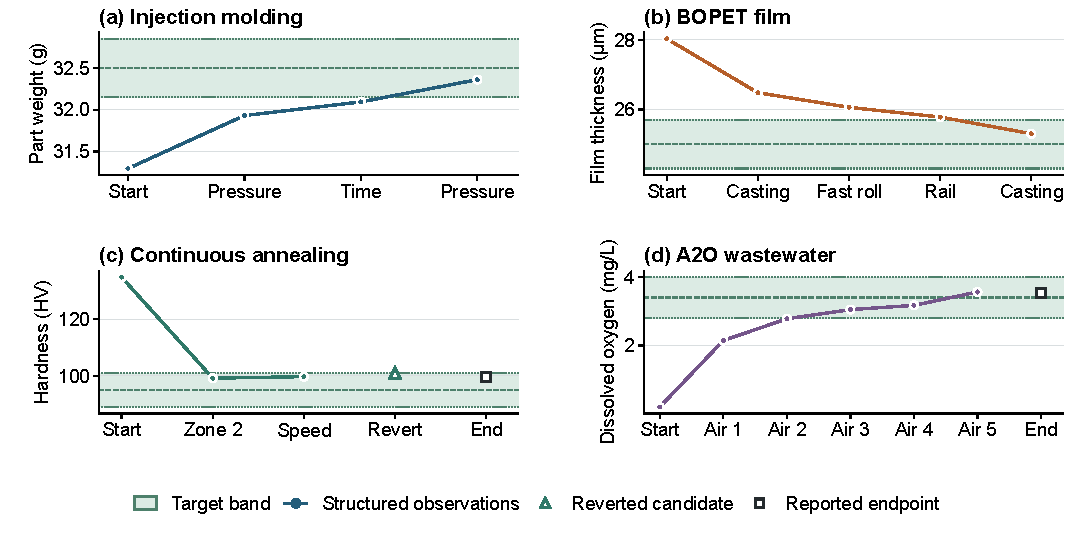
\includegraphics[width=\textwidth]{resources/fig-missions-controls.pdf}
\caption{Process observations from four simulated missions. Shading denotes
the scenario-specific target band and circles denote structured trajectory
observations. The open triangle marks the annealing candidate that was
reverted; its value comes from event text rather than a structured trajectory
record. Open squares show separately reported mission-final values for
annealing and wastewater; these are not connected to the preceding
observations. Horizontal positions indicate event order, not elapsed time.
Each panel represents one deterministic trajectory.}
\label{fig:missions}
\end{figure*}

\subsection{Injection Molding and Film Thickness}
The injection-molding mission sought a part weight of
$32.5\pm0.35$\,g. Starting at 31.296\,g, the routine requested an increase in
holding pressure from 45 to 57.73\,bar, then an increase in holding time from
6 to 10.56\,s. The corresponding observations rose to 31.93 and
32.09\,g. A further pressure request to 62\,bar preceded the final
32.36\,g observation, inside the target band. The record therefore shows
three linked adjustments in one run; it does not isolate the effect of each
parameter through a controlled comparison.

The BOPET mission sought $25.0\pm0.7$\,$\mu$m film thickness. Its initial
observation was 28.03\,$\mu$m. Four requests changed casting speed, fast-roll
speed, rail width, and casting speed again. The successive observations were
26.48, 26.06, 25.78, and 25.30\,$\mu$m. Thus the final value entered the
target band after actions on three controls; the first three observations
remained above the 25.7\,$\mu$m upper limit. The reported melt-temperature
observations during the mission were 291.3--291.8\,$^{\circ}$C, within the
configured 268--300\,$^{\circ}$C window. These measurements characterize
this simulated sequence; they do not establish a general tuning rule for
film lines.

\subsection{Annealing and Wastewater Treatment}
The annealing mission combined a hardness target of $95\pm6$\,HV with a
line-speed increase. The initial hardness was 134.9\,HV. After a zone-2
temperature request from 710 to 850\,$^{\circ}$C, a structured observation
was 99.18\,HV. A speed request from 140 to 152\,m/min was followed by
99.74\,HV. A later 164\,m/min candidate was reverted; the event text reports
101.0\,HV for that candidate, at the upper boundary of the target band.
The mission summary separately reported a final hardness of 99.5\,HV and
retained speed of 152\,m/min. The latter is 8.57\% above the initial
140\,m/min setting, not a measured production-throughput gain. The rejected
candidate reached the upper boundary and failed the configured hardness
margin rule, illustrating why the sequence retained the lower request. The
record also contains a failed zone-3 read
before the zone-2 action. Final tensile-strength and surface-defect
measurements were not archived, so the record cannot establish that all
annealing quality constraints were met.

The wastewater mission first targeted dissolved oxygen (DO) at
$3.4\pm0.6$\,mg/L. Five blower-frequency increases from 26 to 34.1\,Hz
accompanied a rise from 0.194 to 3.567\,mg/L in the structured aeration
sequence. The routine then adjusted alkali and coagulant dosing for pH and
phosphorus, followed by cost-trimming actions. Recorded total-phosphorus
observations fell from 0.662 to 0.5507, 0.4607, and 0.413\,mg/L during dosing.
A later blower reduction was reverted after the recheck found insufficient
margin. The mission separately
reported final DO of 3.54\,mg/L and a change in its simulator-defined cost
index from 182.6 to 180.2. This index is not a measured operating cost. The
complete final effluent vector was not archived; therefore the reported DO
value and cost index do not independently verify all discharge constraints.

\subsection{Evidence Synthesis}
The reported final primary variable lies within its target band in each
mission. The recorded paths differ: molding and film production combine
several actuators, annealing retains a lower-speed setting after a reverted
candidate, and wastewater treatment moves from aeration to chemical dosing.
These examples illustrate how requests and observations can be interpreted
across different simulated objectives. The protocol exercise, onboarding
replay, entry-path checks, and mock approval test address distinct integration and control
questions; their counts are not combined with the four process trajectories.
Together they do not establish
repeatability, causal effects of individual actions, comparative performance,
human-approval effectiveness, or transfer to a physical plant.
